\documentclass[1p]{elsarticle_modified}
%\bibliographystyle{elsarticle-num}

%\usepackage[colorlinks]{hyperref}
%\usepackage{abbrmath_seonhwa} %\Abb, \Ascr, \Acal ,\Abf, \Afrak
\usepackage{amsfonts}
\usepackage{amssymb}
\usepackage{amsmath}
\usepackage{amsthm}
\usepackage{scalefnt}
\usepackage{amsbsy}
\usepackage{kotex}
\usepackage{caption}
\usepackage{subfig}
\usepackage{color}
\usepackage{graphicx}
\usepackage{xcolor} %% white, black, red, green, blue, cyan, magenta, yellow
\usepackage{float}
\usepackage{setspace}
\usepackage{hyperref}

\usepackage{tikz}
\usetikzlibrary{arrows}

\usepackage{multirow}
\usepackage{array} % fixed length table
\usepackage{hhline}

%%%%%%%%%%%%%%%%%%%%%
\makeatletter
\renewcommand*\env@matrix[1][\arraystretch]{%
	\edef\arraystretch{#1}%
	\hskip -\arraycolsep
	\let\@ifnextchar\new@ifnextchar
	\array{*\c@MaxMatrixCols c}}
\makeatother %https://tex.stackexchange.com/questions/14071/how-can-i-increase-the-line-spacing-in-a-matrix
%%%%%%%%%%%%%%%

\usepackage[normalem]{ulem}

\newcommand{\msout}[1]{\ifmmode\text{\sout{\ensuremath{#1}}}\else\sout{#1}\fi}
%SOURCE: \msout is \stkout macro in https://tex.stackexchange.com/questions/20609/strikeout-in-math-mode

\newcommand{\cancel}[1]{
	\ifmmode
	{\color{red}\msout{#1}}
	\else
	{\color{red}\sout{#1}}
	\fi
}

\newcommand{\add}[1]{
	{\color{blue}\uwave{#1}}
}

\newcommand{\replace}[2]{
	\ifmmode
	{\color{red}\msout{#1}}{\color{blue}\uwave{#2}}
	\else
	{\color{red}\sout{#1}}{\color{blue}\uwave{#2}}
	\fi
}

\newcommand{\Sol}{\mathcal{S}} %segment
\newcommand{\D}{D} %diagram
\newcommand{\A}{\mathcal{A}} %arc


%%%%%%%%%%%%%%%%%%%%%%%%%%%%%5 test

\def\sl{\operatorname{\textup{SL}}(2,\Cbb)}
\def\psl{\operatorname{\textup{PSL}}(2,\Cbb)}
\def\quan{\mkern 1mu \triangleright \mkern 1mu}

\theoremstyle{definition}
\newtheorem{thm}{Theorem}[section]
\newtheorem{prop}[thm]{Proposition}
\newtheorem{lem}[thm]{Lemma}
\newtheorem{ques}[thm]{Question}
\newtheorem{cor}[thm]{Corollary}
\newtheorem{defn}[thm]{Definition}
\newtheorem{exam}[thm]{Example}
\newtheorem{rmk}[thm]{Remark}
\newtheorem{alg}[thm]{Algorithm}

\newcommand{\I}{\sqrt{-1}}
\begin{document}

%\begin{frontmatter}
%
%\title{Boundary parabolic representations of knots up to 8 crossings}
%
%%% Group authors per affiliation:
%\author{Yunhi Cho} 
%\address{Department of Mathematics, University of Seoul, Seoul, Korea}
%\ead{yhcho@uos.ac.kr}
%
%
%\author{Seonhwa Kim} %\fnref{s_kim}}
%\address{Center for Geometry and Physics, Institute for Basic Science, Pohang, 37673, Korea}
%\ead{ryeona17@ibs.re.kr}
%
%\author{Hyuk Kim}
%\address{Department of Mathematical Sciences, Seoul National University, Seoul 08826, Korea}
%\ead{hyukkim@snu.ac.kr}
%
%\author{Seokbeom Yoon}
%\address{Department of Mathematical Sciences, Seoul National University, Seoul, 08826,  Korea}
%\ead{sbyoon15@snu.ac.kr}
%
%\begin{abstract}
%We find all boundary parabolic representation of knots up to 8 crossings.
%
%\end{abstract}
%\begin{keyword}
%    \MSC[2010] 57M25 
%\end{keyword}
%
%\end{frontmatter}

%\linenumbers
%\tableofcontents
%
\newcommand\colored[1]{\textcolor{white}{\rule[-0.35ex]{0.8em}{1.4ex}}\kern-0.8em\color{red} #1}%
%\newcommand\colored[1]{\textcolor{white}{ #1}\kern-2.17ex	\textcolor{white}{ #1}\kern-1.81ex	\textcolor{white}{ #1}\kern-2.15ex\color{red}#1	}

{\Large $\underline{12a_{0873}~(K12a_{0873})}$}

\setlength{\tabcolsep}{10pt}
\renewcommand{\arraystretch}{1.6}
\vspace{1cm}\begin{tabular}{m{100pt}>{\centering\arraybackslash}m{274pt}}
\multirow{5}{120pt}{
	\centering
	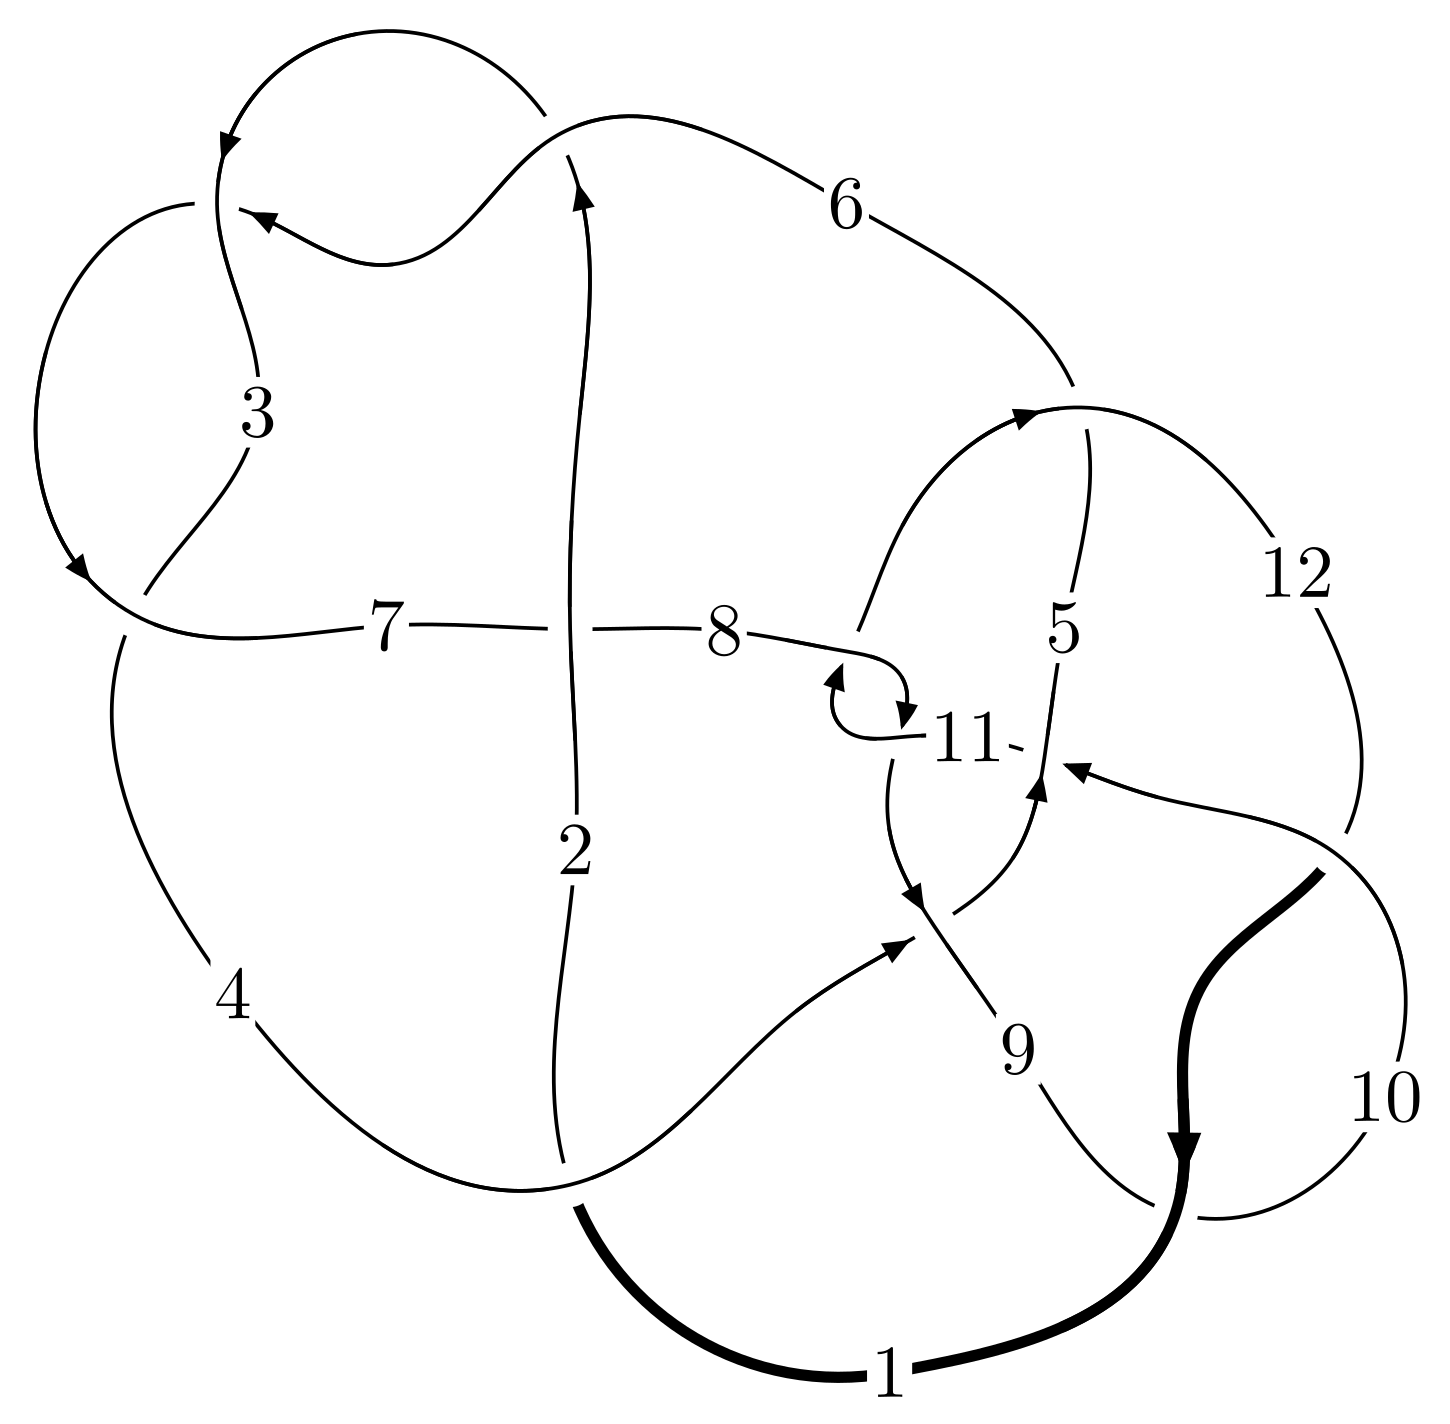
\includegraphics[width=112pt]{../../../GIT/diagram.site/Diagrams/png/1674_12a_0873.png}\\
\ \ \ A knot diagram\footnotemark}&
\allowdisplaybreaks
\textbf{Linearized knot diagam} \\
\cline{2-2}
 &
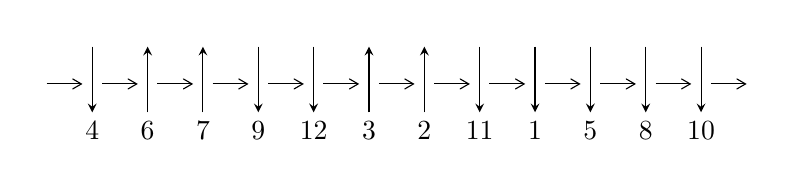
\begin{tikzpicture}[x=20pt, y=17pt]
	% nodes
	\node (C0) at (0, 0) {};
	\node (C1) at (1, 0) {};
	\node (C1U) at (1, +1) {};
	\node (C1D) at (1, -1) {4};

	\node (C2) at (2, 0) {};
	\node (C2U) at (2, +1) {};
	\node (C2D) at (2, -1) {6};

	\node (C3) at (3, 0) {};
	\node (C3U) at (3, +1) {};
	\node (C3D) at (3, -1) {7};

	\node (C4) at (4, 0) {};
	\node (C4U) at (4, +1) {};
	\node (C4D) at (4, -1) {9};

	\node (C5) at (5, 0) {};
	\node (C5U) at (5, +1) {};
	\node (C5D) at (5, -1) {12};

	\node (C6) at (6, 0) {};
	\node (C6U) at (6, +1) {};
	\node (C6D) at (6, -1) {3};

	\node (C7) at (7, 0) {};
	\node (C7U) at (7, +1) {};
	\node (C7D) at (7, -1) {2};

	\node (C8) at (8, 0) {};
	\node (C8U) at (8, +1) {};
	\node (C8D) at (8, -1) {11};

	\node (C9) at (9, 0) {};
	\node (C9U) at (9, +1) {};
	\node (C9D) at (9, -1) {1};

	\node (C10) at (10, 0) {};
	\node (C10U) at (10, +1) {};
	\node (C10D) at (10, -1) {5};

	\node (C11) at (11, 0) {};
	\node (C11U) at (11, +1) {};
	\node (C11D) at (11, -1) {8};

	\node (C12) at (12, 0) {};
	\node (C12U) at (12, +1) {};
	\node (C12D) at (12, -1) {10};
	\node (C13) at (13, 0) {};

	% arrows
	\draw[->,>={angle 60}]
	(C0) edge (C1) (C1) edge (C2) (C2) edge (C3) (C3) edge (C4) (C4) edge (C5) (C5) edge (C6) (C6) edge (C7) (C7) edge (C8) (C8) edge (C9) (C9) edge (C10) (C10) edge (C11) (C11) edge (C12) (C12) edge (C13) ;	\draw[->,>=stealth]
	(C1U) edge (C1D) (C2D) edge (C2U) (C3D) edge (C3U) (C4U) edge (C4D) (C5U) edge (C5D) (C6D) edge (C6U) (C7D) edge (C7U) (C8U) edge (C8D) (C9U) edge (C9D) (C10U) edge (C10D) (C11U) edge (C11D) (C12U) edge (C12D) ;
	\end{tikzpicture} \\
\hhline{~~} \\& 
\textbf{Solving Sequence} \\ \cline{2-2} 
 &
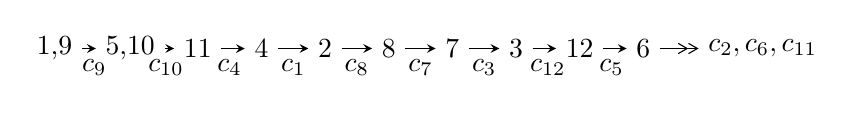
\begin{tikzpicture}[x=23pt, y=7pt]
	% node
	\node (A0) at (-1/8, 0) {1,9};
	\node (A1) at (17/16, 0) {5,10};
	\node (A2) at (17/8, 0) {11};
	\node (A3) at (25/8, 0) {4};
	\node (A4) at (33/8, 0) {2};
	\node (A5) at (41/8, 0) {8};
	\node (A6) at (49/8, 0) {7};
	\node (A7) at (57/8, 0) {3};
	\node (A8) at (65/8, 0) {12};
	\node (A9) at (73/8, 0) {6};
	\node (C1) at (1/2, -1) {$c_{9}$};
	\node (C2) at (13/8, -1) {$c_{10}$};
	\node (C3) at (21/8, -1) {$c_{4}$};
	\node (C4) at (29/8, -1) {$c_{1}$};
	\node (C5) at (37/8, -1) {$c_{8}$};
	\node (C6) at (45/8, -1) {$c_{7}$};
	\node (C7) at (53/8, -1) {$c_{3}$};
	\node (C8) at (61/8, -1) {$c_{12}$};
	\node (C9) at (69/8, -1) {$c_{5}$};
	\node (A10) at (11, 0) {$c_{2},c_{6},c_{11}$};

	% edge
	\draw[->,>=stealth]	
	(A0) edge (A1) (A1) edge (A2) (A2) edge (A3) (A3) edge (A4) (A4) edge (A5) (A5) edge (A6) (A6) edge (A7) (A7) edge (A8) (A8) edge (A9) ;
	\draw[->>,>={angle 60}]	
	(A9) edge (A10);
\end{tikzpicture} \\ 

\end{tabular} \\

\footnotetext{
The image of knot diagram is generated by the software ``\textbf{Draw programme}" developed by Andrew Bartholomew(\url{http://www.layer8.co.uk/maths/draw/index.htm\#Running-draw}), where we modified some parts for our purpose(\url{https://github.com/CATsTAILs/LinksPainter}).
}\phantom \\ \newline 
\centering \textbf{Ideals for irreducible components\footnotemark of $X_{\text{par}}$} 
 
\begin{align*}
I^u_{1}&=\langle 
108691 u^{38}-518522 u^{37}+\cdots+524288 b-511627,\\
\phantom{I^u_{1}}&\phantom{= \langle  }688007 u^{38}-3615026 u^{37}+\cdots+524288 a-2014079,\;u^{39}-5 u^{38}+\cdots-6 u-1\rangle \\
I^u_{2}&=\langle 
6.85428\times10^{68} u^{61}+3.56097\times10^{69} u^{60}+\cdots+4.46626\times10^{69} b-6.45538\times10^{69},\\
\phantom{I^u_{2}}&\phantom{= \langle  }-3.56475\times10^{68} u^{61}-1.48838\times10^{68} u^{60}+\cdots+4.46626\times10^{69} a+1.70079\times10^{70},\\
\phantom{I^u_{2}}&\phantom{= \langle  }u^{62}+11 u^{61}+\cdots+11 u+2\rangle \\
I^u_{3}&=\langle 
b- a,\;32 a^5-16 a^4+16 a^3-4 a^2+2 a-1,\;u-1\rangle \\
I^u_{4}&=\langle 
b- u-1,\;a+2 u+1,\;u^2+1\rangle \\
\\
\end{align*}
\raggedright * 4 irreducible components of $\dim_{\mathbb{C}}=0$, with total 108 representations.\\
\footnotetext{All coefficients of polynomials are rational numbers. But the coefficients are sometimes approximated in decimal forms when there is not enough margin.}
\newpage
\renewcommand{\arraystretch}{1}
\centering \section*{I. $I^u_{1}= \langle 1.09\times10^{5} u^{38}-5.19\times10^{5} u^{37}+\cdots+5.24\times10^{5} b-5.12\times10^{5},\;6.88\times10^{5} u^{38}-3.62\times10^{6} u^{37}+\cdots+5.24\times10^{5} a-2.01\times10^{6},\;u^{39}-5 u^{38}+\cdots-6 u-1 \rangle$}
\flushleft \textbf{(i) Arc colorings}\\
\begin{tabular}{m{7pt} m{180pt} m{7pt} m{180pt} }
\flushright $a_{1}=$&$\begin{pmatrix}0\\u\end{pmatrix}$ \\
\flushright $a_{9}=$&$\begin{pmatrix}1\\0\end{pmatrix}$ \\
\flushright $a_{5}=$&$\begin{pmatrix}-1.31227 u^{38}+6.89511 u^{37}+\cdots+14.1550 u+3.84155\\-0.207312 u^{38}+0.989002 u^{37}+\cdots+2.65564 u+0.975851\end{pmatrix}$ \\
\flushright $a_{10}=$&$\begin{pmatrix}1\\u^2\end{pmatrix}$ \\
\flushright $a_{11}=$&$\begin{pmatrix}-\frac{1}{8} u^{37}+\frac{5}{8} u^{36}+\cdots+\frac{11}{4} u+\frac{1}{8}\\u\end{pmatrix}$ \\
\flushright $a_{4}=$&$\begin{pmatrix}-1.51958 u^{38}+7.88412 u^{37}+\cdots+16.8107 u+4.81740\\-0.207312 u^{38}+0.989002 u^{37}+\cdots+2.65564 u+0.975851\end{pmatrix}$ \\
\flushright $a_{2}=$&$\begin{pmatrix}0.124998 u^{38}-0.624989 u^{37}+\cdots+5.87501 u-0.999998\\-9.53674\times10^{-7} u^{38}+5.72205\times10^{-6} u^{37}+\cdots+2.00000 u+9.53674\times10^{-7}\end{pmatrix}$ \\
\flushright $a_{8}=$&$\begin{pmatrix}\frac{1}{8} u^{38}-\frac{5}{8} u^{37}+\cdots-\frac{1}{8} u+1\\- u^2\end{pmatrix}$ \\
\flushright $a_{7}=$&$\begin{pmatrix}0.125425 u^{38}-0.627522 u^{37}+\cdots-2.12725 u+0.999544\\0.000203133 u^{38}-0.00120354 u^{37}+\cdots-0.00107670 u-0.000218391\end{pmatrix}$ \\
\flushright $a_{3}=$&$\begin{pmatrix}-0.000410080 u^{38}+0.00242996 u^{37}+\cdots+4.00217 u+0.000440598\\-0.000540733 u^{38}+0.00319862 u^{37}+\cdots+1.00289 u+0.000586510\end{pmatrix}$ \\
\flushright $a_{12}=$&$\begin{pmatrix}u\\u^3+u\end{pmatrix}$ \\
\flushright $a_{6}=$&$\begin{pmatrix}-1.26471 u^{38}+6.61468 u^{37}+\cdots+14.4231 u+4.04886\\-0.315355 u^{38}+1.65487 u^{37}+\cdots+2.71527 u+1.14050\end{pmatrix}$\\&\end{tabular}
\flushleft \textbf{(ii) Obstruction class $= -1$}\\~\\
\flushleft \textbf{(iii) Cusp Shapes $= -\frac{3999055}{2097152} u^{38}+\frac{10274157}{1048576} u^{37}+\cdots+\frac{37199499}{2097152} u+\frac{9939535}{2097152}$}\\~\\
\newpage\renewcommand{\arraystretch}{1}
\flushleft \textbf{(iv) u-Polynomials at the component}\newline \\
\begin{tabular}{m{50pt}|m{274pt}}
Crossings & \hspace{64pt}u-Polynomials at each crossing \\
\hline $$\begin{aligned}c_{1}\end{aligned}$$&$\begin{aligned}
&u^{39}-8 u^{38}+\cdots+78583 u-7136
\end{aligned}$\\
\hline $$\begin{aligned}c_{2},c_{3},c_{6}\end{aligned}$$&$\begin{aligned}
&u^{39}-2 u^{38}+\cdots+13 u+4
\end{aligned}$\\
\hline $$\begin{aligned}c_{4},c_{5}\end{aligned}$$&$\begin{aligned}
&32(32 u^{39}-16 u^{38}+\cdots+2 u+2)
\end{aligned}$\\
\hline $$\begin{aligned}c_{7}\end{aligned}$$&$\begin{aligned}
&u^{39}-5 u^{37}+\cdots+3664 u+704
\end{aligned}$\\
\hline $$\begin{aligned}c_{8},c_{9},c_{11}\\c_{12}\end{aligned}$$&$\begin{aligned}
&u^{39}+5 u^{38}+\cdots-6 u+1
\end{aligned}$\\
\hline $$\begin{aligned}c_{10}\end{aligned}$$&$\begin{aligned}
&u^{39}+3 u^{38}+\cdots+5632 u+2048
\end{aligned}$\\
\hline
\end{tabular}\\~\\
\newpage\renewcommand{\arraystretch}{1}
\flushleft \textbf{(v) Riley Polynomials at the component}\newline \\
\begin{tabular}{m{50pt}|m{274pt}}
Crossings & \hspace{64pt}Riley Polynomials at each crossing \\
\hline $$\begin{aligned}c_{1}\end{aligned}$$&$\begin{aligned}
&y^{39}+24 y^{38}+\cdots+2799146385 y-50922496
\end{aligned}$\\
\hline $$\begin{aligned}c_{2},c_{3},c_{6}\end{aligned}$$&$\begin{aligned}
&y^{39}-36 y^{38}+\cdots+145 y-16
\end{aligned}$\\
\hline $$\begin{aligned}c_{4},c_{5}\end{aligned}$$&$\begin{aligned}
&1024(1024 y^{39}+21248 y^{38}+\cdots-20 y-4)
\end{aligned}$\\
\hline $$\begin{aligned}c_{7}\end{aligned}$$&$\begin{aligned}
&y^{39}-10 y^{38}+\cdots+9786624 y-495616
\end{aligned}$\\
\hline $$\begin{aligned}c_{8},c_{9},c_{11}\\c_{12}\end{aligned}$$&$\begin{aligned}
&y^{39}+23 y^{38}+\cdots+16 y-1
\end{aligned}$\\
\hline $$\begin{aligned}c_{10}\end{aligned}$$&$\begin{aligned}
&y^{39}+13 y^{38}+\cdots-77332480 y-4194304
\end{aligned}$\\
\hline
\end{tabular}\\~\\
\newpage\flushleft \textbf{(vi) Complex Volumes and Cusp Shapes}
$$\begin{array}{c|c|c}  
\text{Solutions to }I^u_{1}& \I (\text{vol} + \sqrt{-1}CS) & \text{Cusp shape}\\
 \hline 
\begin{aligned}
u &= \phantom{-}0.724185 + 0.655758 I \\
a &= \phantom{-}0.330095 + 0.170004 I \\
b &= \phantom{-}0.738223 - 0.031571 I\end{aligned}
 & \phantom{-}2.17537 - 4.39053 I & -3.44910 + 4.97696 I \\ \hline\begin{aligned}
u &= \phantom{-}0.724185 - 0.655758 I \\
a &= \phantom{-}0.330095 - 0.170004 I \\
b &= \phantom{-}0.738223 + 0.031571 I\end{aligned}
 & \phantom{-}2.17537 + 4.39053 I & -3.44910 - 4.97696 I \\ \hline\begin{aligned}
u &= \phantom{-}0.798846 + 0.475502 I \\
a &= -0.164314 - 0.150407 I \\
b &= -0.630420 + 0.127305 I\end{aligned}
 & -2.50450 - 1.68373 I & -12.13938 + 2.32742 I \\ \hline\begin{aligned}
u &= \phantom{-}0.798846 - 0.475502 I \\
a &= -0.164314 + 0.150407 I \\
b &= -0.630420 - 0.127305 I\end{aligned}
 & -2.50450 + 1.68373 I & -12.13938 - 2.32742 I \\ \hline\begin{aligned}
u &= \phantom{-}1.066700 + 0.355106 I \\
a &= \phantom{-}0.0961583 + 0.0078123 I \\
b &= \phantom{-}0.524239 - 0.376281 I\end{aligned}
 & \phantom{-}0.475249 + 0.503953 I & -4.00000 - 8.90257 I \\ \hline\begin{aligned}
u &= \phantom{-}1.066700 - 0.355106 I \\
a &= \phantom{-}0.0961583 - 0.0078123 I \\
b &= \phantom{-}0.524239 + 0.376281 I\end{aligned}
 & \phantom{-}0.475249 - 0.503953 I & -4.00000 + 8.90257 I \\ \hline\begin{aligned}
u &= -0.211517 + 1.137440 I \\
a &= \phantom{-}0.23998 - 2.28740 I \\
b &= -0.464258 + 0.732877 I\end{aligned}
 & \phantom{-}5.31272 + 2.00033 I & \phantom{-}4.35226 - 5.73915 I \\ \hline\begin{aligned}
u &= -0.211517 - 1.137440 I \\
a &= \phantom{-}0.23998 + 2.28740 I \\
b &= -0.464258 - 0.732877 I\end{aligned}
 & \phantom{-}5.31272 - 2.00033 I & \phantom{-}4.35226 + 5.73915 I \\ \hline\begin{aligned}
u &= -0.324360 + 1.156690 I \\
a &= \phantom{-}0.02796 + 2.07352 I \\
b &= \phantom{-}0.697354 - 0.867496 I\end{aligned}
 & \phantom{-}2.21977 + 6.32089 I & \phantom{-0.000000 } 0. - 7.80217 I \\ \hline\begin{aligned}
u &= -0.324360 - 1.156690 I \\
a &= \phantom{-}0.02796 - 2.07352 I \\
b &= \phantom{-}0.697354 + 0.867496 I\end{aligned}
 & \phantom{-}2.21977 - 6.32089 I & \phantom{-0.000000 -}0. + 7.80217 I\\
 \hline 
 \end{array}$$\newpage$$\begin{array}{c|c|c}  
\text{Solutions to }I^u_{1}& \I (\text{vol} + \sqrt{-1}CS) & \text{Cusp shape}\\
 \hline 
\begin{aligned}
u &= \phantom{-}0.026900 + 1.214660 I \\
a &= \phantom{-}1.23416 - 1.59634 I \\
b &= \phantom{-}0.132335 + 0.743058 I\end{aligned}
 & \phantom{-}7.44405 + 0.69867 I & \phantom{-}9.09911 + 0. I\phantom{ +0.000000I} \\ \hline\begin{aligned}
u &= \phantom{-}0.026900 - 1.214660 I \\
a &= \phantom{-}1.23416 + 1.59634 I \\
b &= \phantom{-}0.132335 - 0.743058 I\end{aligned}
 & \phantom{-}7.44405 - 0.69867 I & \phantom{-}9.09911 + 0. I\phantom{ +0.000000I} \\ \hline\begin{aligned}
u &= \phantom{-}0.122259 + 1.210610 I \\
a &= -1.34335 + 1.13263 I \\
b &= -0.327572 - 0.697824 I\end{aligned}
 & \phantom{-}6.47328 - 4.27244 I & \phantom{-0.000000 } 0 \\ \hline\begin{aligned}
u &= \phantom{-}0.122259 - 1.210610 I \\
a &= -1.34335 - 1.13263 I \\
b &= -0.327572 + 0.697824 I\end{aligned}
 & \phantom{-}6.47328 + 4.27244 I & \phantom{-0.000000 } 0 \\ \hline\begin{aligned}
u &= \phantom{-}0.182168 + 1.256440 I \\
a &= \phantom{-}1.13163 - 0.93796 I \\
b &= \phantom{-}0.456095 + 0.759995 I\end{aligned}
 & \phantom{-}12.6122 - 8.2561 I & \phantom{-0.000000 } 0 \\ \hline\begin{aligned}
u &= \phantom{-}0.182168 - 1.256440 I \\
a &= \phantom{-}1.13163 + 0.93796 I \\
b &= \phantom{-}0.456095 - 0.759995 I\end{aligned}
 & \phantom{-}12.6122 + 8.2561 I & \phantom{-0.000000 } 0 \\ \hline\begin{aligned}
u &= -0.407095 + 1.204330 I \\
a &= -0.13247 - 1.90492 I \\
b &= -0.843449 + 1.039000 I\end{aligned}
 & \phantom{-}6.42042 + 10.35860 I & \phantom{-0.000000 } 0 \\ \hline\begin{aligned}
u &= -0.407095 - 1.204330 I \\
a &= -0.13247 + 1.90492 I \\
b &= -0.843449 - 1.039000 I\end{aligned}
 & \phantom{-}6.42042 - 10.35860 I & \phantom{-0.000000 } 0 \\ \hline\begin{aligned}
u &= \phantom{-}1.319840 + 0.082124 I \\
a &= -0.0186151 + 0.0626784 I \\
b &= -0.127627 + 0.707014 I\end{aligned}
 & -0.85359 + 1.74269 I & \phantom{-0.000000 } 0 \\ \hline\begin{aligned}
u &= \phantom{-}1.319840 - 0.082124 I \\
a &= -0.0186151 - 0.0626784 I \\
b &= -0.127627 - 0.707014 I\end{aligned}
 & -0.85359 - 1.74269 I & \phantom{-0.000000 } 0\\
 \hline 
 \end{array}$$\newpage$$\begin{array}{c|c|c}  
\text{Solutions to }I^u_{1}& \I (\text{vol} + \sqrt{-1}CS) & \text{Cusp shape}\\
 \hline 
\begin{aligned}
u &= -0.036557 + 1.324810 I \\
a &= -0.73447 + 1.53147 I \\
b &= -0.062358 - 1.015090 I\end{aligned}
 & \phantom{-}15.0323 + 3.2046 I & \phantom{-0.000000 } 0 \\ \hline\begin{aligned}
u &= -0.036557 - 1.324810 I \\
a &= -0.73447 - 1.53147 I \\
b &= -0.062358 + 1.015090 I\end{aligned}
 & \phantom{-}15.0323 - 3.2046 I & \phantom{-0.000000 } 0 \\ \hline\begin{aligned}
u &= \phantom{-}0.594439\phantom{ +0.000000I} \\
a &= -0.228045\phantom{ +0.000000I} \\
b &= \phantom{-}0.452360\phantom{ +0.000000I}\end{aligned}
 & -0.941763\phantom{ +0.000000I} & -9.94040\phantom{ +0.000000I} \\ \hline\begin{aligned}
u &= \phantom{-}1.41463 + 0.10708 I \\
a &= \phantom{-}0.0231744 - 0.0841694 I \\
b &= \phantom{-}0.166254 - 0.853051 I\end{aligned}
 & \phantom{-}4.93767 + 4.69901 I & \phantom{-0.000000 } 0 \\ \hline\begin{aligned}
u &= \phantom{-}1.41463 - 0.10708 I \\
a &= \phantom{-}0.0231744 + 0.0841694 I \\
b &= \phantom{-}0.166254 + 0.853051 I\end{aligned}
 & \phantom{-}4.93767 - 4.69901 I & \phantom{-0.000000 } 0 \\ \hline\begin{aligned}
u &= -0.47769 + 1.37991 I \\
a &= -0.14495 - 1.60254 I \\
b &= -0.85620 + 1.49381 I\end{aligned}
 & \phantom{-}9.12652 + 9.53608 I & \phantom{-0.000000 } 0 \\ \hline\begin{aligned}
u &= -0.47769 - 1.37991 I \\
a &= -0.14495 + 1.60254 I \\
b &= -0.85620 - 1.49381 I\end{aligned}
 & \phantom{-}9.12652 - 9.53608 I & \phantom{-0.000000 } 0 \\ \hline\begin{aligned}
u &= -0.52260 + 1.38710 I \\
a &= \phantom{-}0.20032 + 1.57749 I \\
b &= \phantom{-}0.95190 - 1.54963 I\end{aligned}
 & \phantom{-}8.2828 + 13.9866 I & \phantom{-0.000000 } 0 \\ \hline\begin{aligned}
u &= -0.52260 - 1.38710 I \\
a &= \phantom{-}0.20032 - 1.57749 I \\
b &= \phantom{-}0.95190 + 1.54963 I\end{aligned}
 & \phantom{-}8.2828 - 13.9866 I & \phantom{-0.000000 } 0 \\ \hline\begin{aligned}
u &= -0.43911 + 1.42736 I \\
a &= \phantom{-}0.08082 + 1.54888 I \\
b &= \phantom{-}0.72748 - 1.56656 I\end{aligned}
 & \phantom{-}16.0878 + 7.0331 I & \phantom{-0.000000 } 0\\
 \hline 
 \end{array}$$\newpage$$\begin{array}{c|c|c}  
\text{Solutions to }I^u_{1}& \I (\text{vol} + \sqrt{-1}CS) & \text{Cusp shape}\\
 \hline 
\begin{aligned}
u &= -0.43911 - 1.42736 I \\
a &= \phantom{-}0.08082 - 1.54888 I \\
b &= \phantom{-}0.72748 + 1.56656 I\end{aligned}
 & \phantom{-}16.0878 - 7.0331 I & \phantom{-0.000000 } 0 \\ \hline\begin{aligned}
u &= -0.54482 + 1.40917 I \\
a &= -0.21934 - 1.54269 I \\
b &= -0.98301 + 1.61986 I\end{aligned}
 & \phantom{-}14.2175 + 17.6988 I & \phantom{-0.000000 } 0 \\ \hline\begin{aligned}
u &= -0.54482 - 1.40917 I \\
a &= -0.21934 + 1.54269 I \\
b &= -0.98301 - 1.61986 I\end{aligned}
 & \phantom{-}14.2175 - 17.6988 I & \phantom{-0.000000 } 0 \\ \hline\begin{aligned}
u &= \phantom{-}0.015211 + 0.418244 I \\
a &= -0.00352 - 1.79696 I \\
b &= -0.539074 - 0.214516 I\end{aligned}
 & \phantom{-}2.76604 + 0.58348 I & -0.871646 + 0.155316 I \\ \hline\begin{aligned}
u &= \phantom{-}0.015211 - 0.418244 I \\
a &= -0.00352 + 1.79696 I \\
b &= -0.539074 + 0.214516 I\end{aligned}
 & \phantom{-}2.76604 - 0.58348 I & -0.871646 - 0.155316 I \\ \hline\begin{aligned}
u &= -0.310457 + 0.116493 I \\
a &= -0.01154 - 3.00812 I \\
b &= -0.275051 - 0.775463 I\end{aligned}
 & \phantom{-}5.36389 - 4.18845 I & \phantom{-}5.68066 + 2.80926 I \\ \hline\begin{aligned}
u &= -0.310457 - 0.116493 I \\
a &= -0.01154 + 3.00812 I \\
b &= -0.275051 + 0.775463 I\end{aligned}
 & \phantom{-}5.36389 + 4.18845 I & \phantom{-}5.68066 - 2.80926 I \\ \hline\begin{aligned}
u &= -0.193758 + 0.118859 I \\
a &= -0.22771 + 3.00764 I \\
b &= \phantom{-}0.238959 + 0.534501 I\end{aligned}
 & \phantom{-}0.026832 - 1.339450 I & \phantom{-}0.33272 + 4.35005 I \\ \hline\begin{aligned}
u &= -0.193758 - 0.118859 I \\
a &= -0.22771 - 3.00764 I \\
b &= \phantom{-}0.238959 - 0.534501 I\end{aligned}
 & \phantom{-}0.026832 + 1.339450 I & \phantom{-}0.33272 - 4.35005 I\\
 \hline 
 \end{array}$$\newpage\newpage\renewcommand{\arraystretch}{1}
\centering \section*{II. $I^u_{2}= \langle 6.85\times10^{68} u^{61}+3.56\times10^{69} u^{60}+\cdots+4.47\times10^{69} b-6.46\times10^{69},\;-3.56\times10^{68} u^{61}-1.49\times10^{68} u^{60}+\cdots+4.47\times10^{69} a+1.70\times10^{70},\;u^{62}+11 u^{61}+\cdots+11 u+2 \rangle$}
\flushleft \textbf{(i) Arc colorings}\\
\begin{tabular}{m{7pt} m{180pt} m{7pt} m{180pt} }
\flushright $a_{1}=$&$\begin{pmatrix}0\\u\end{pmatrix}$ \\
\flushright $a_{9}=$&$\begin{pmatrix}1\\0\end{pmatrix}$ \\
\flushright $a_{5}=$&$\begin{pmatrix}0.0798151 u^{61}+0.0333250 u^{60}+\cdots-20.7102 u-3.80808\\-0.153468 u^{61}-0.797304 u^{60}+\cdots+10.2193 u+1.44537\end{pmatrix}$ \\
\flushright $a_{10}=$&$\begin{pmatrix}1\\u^2\end{pmatrix}$ \\
\flushright $a_{11}=$&$\begin{pmatrix}\frac{1}{2} u^{61}+\frac{11}{2} u^{60}+\cdots+\frac{45}{2} u+\frac{11}{2}\\0.573998 u^{61}+5.87664 u^{60}+\cdots+1.67615 u+0.498297\end{pmatrix}$ \\
\flushright $a_{4}=$&$\begin{pmatrix}-0.0736529 u^{61}-0.763979 u^{60}+\cdots-10.4908 u-2.36271\\-0.153468 u^{61}-0.797304 u^{60}+\cdots+10.2193 u+1.44537\end{pmatrix}$ \\
\flushright $a_{2}=$&$\begin{pmatrix}0.636727 u^{61}+7.29918 u^{60}+\cdots+7.35507 u+2.59664\\0.175214 u^{61}+2.55480 u^{60}+\cdots+10.5476 u+2.81253\end{pmatrix}$ \\
\flushright $a_{8}=$&$\begin{pmatrix}-0.249149 u^{61}-2.16664 u^{60}+\cdots-0.729108 u-0.0644857\\-0.437334 u^{61}-4.84227 u^{60}+\cdots-5.81568 u-0.147996\end{pmatrix}$ \\
\flushright $a_{7}=$&$\begin{pmatrix}-0.0660678 u^{61}-0.546435 u^{60}+\cdots+9.22039 u+2.55081\\-0.00796357 u^{61}-0.597986 u^{60}+\cdots-8.29547 u-1.03845\end{pmatrix}$ \\
\flushright $a_{3}=$&$\begin{pmatrix}0.127793 u^{61}+1.67388 u^{60}+\cdots-0.711897 u+0.745056\\-0.0486349 u^{61}+0.0587942 u^{60}+\cdots+8.88154 u+1.74770\end{pmatrix}$ \\
\flushright $a_{12}=$&$\begin{pmatrix}u\\u^3+u\end{pmatrix}$ \\
\flushright $a_{6}=$&$\begin{pmatrix}-0.118114 u^{61}-1.24898 u^{60}+\cdots-12.0046 u-2.25218\\-0.157786 u^{61}-1.09012 u^{60}+\cdots+9.47656 u+1.21142\end{pmatrix}$\\&\end{tabular}
\flushleft \textbf{(ii) Obstruction class $= -1$}\\~\\
\flushleft \textbf{(iii) Cusp Shapes $= -1.03298 u^{61}-9.77347 u^{60}+\cdots-1.48702 u-3.35758$}\\~\\
\newpage\renewcommand{\arraystretch}{1}
\flushleft \textbf{(iv) u-Polynomials at the component}\newline \\
\begin{tabular}{m{50pt}|m{274pt}}
Crossings & \hspace{64pt}u-Polynomials at each crossing \\
\hline $$\begin{aligned}c_{1}\end{aligned}$$&$\begin{aligned}
&(u^{31}-5 u^{30}+\cdots+40 u-7)^{2}
\end{aligned}$\\
\hline $$\begin{aligned}c_{2},c_{3},c_{6}\end{aligned}$$&$\begin{aligned}
&(u^{31}- u^{30}+\cdots+2 u-1)^{2}
\end{aligned}$\\
\hline $$\begin{aligned}c_{4},c_{5}\end{aligned}$$&$\begin{aligned}
&u^{62}+u^{61}+\cdots-768736 u+1008568
\end{aligned}$\\
\hline $$\begin{aligned}c_{7}\end{aligned}$$&$\begin{aligned}
&(u^{31}+3 u^{30}+\cdots-13 u+16)^{2}
\end{aligned}$\\
\hline $$\begin{aligned}c_{8},c_{9},c_{11}\\c_{12}\end{aligned}$$&$\begin{aligned}
&u^{62}-11 u^{61}+\cdots-11 u+2
\end{aligned}$\\
\hline $$\begin{aligned}c_{10}\end{aligned}$$&$\begin{aligned}
&(u^{31}- u^{30}+\cdots+2 u^2+1)^{2}
\end{aligned}$\\
\hline
\end{tabular}\\~\\
\newpage\renewcommand{\arraystretch}{1}
\flushleft \textbf{(v) Riley Polynomials at the component}\newline \\
\begin{tabular}{m{50pt}|m{274pt}}
Crossings & \hspace{64pt}Riley Polynomials at each crossing \\
\hline $$\begin{aligned}c_{1}\end{aligned}$$&$\begin{aligned}
&(y^{31}+23 y^{30}+\cdots-640 y-49)^{2}
\end{aligned}$\\
\hline $$\begin{aligned}c_{2},c_{3},c_{6}\end{aligned}$$&$\begin{aligned}
&(y^{31}-29 y^{30}+\cdots-4 y-1)^{2}
\end{aligned}$\\
\hline $$\begin{aligned}c_{4},c_{5}\end{aligned}$$&$\begin{aligned}
&y^{62}+35 y^{61}+\cdots+17185261710176 y+1017209410624
\end{aligned}$\\
\hline $$\begin{aligned}c_{7}\end{aligned}$$&$\begin{aligned}
&(y^{31}-9 y^{30}+\cdots+1481 y-256)^{2}
\end{aligned}$\\
\hline $$\begin{aligned}c_{8},c_{9},c_{11}\\c_{12}\end{aligned}$$&$\begin{aligned}
&y^{62}+43 y^{61}+\cdots+59 y+4
\end{aligned}$\\
\hline $$\begin{aligned}c_{10}\end{aligned}$$&$\begin{aligned}
&(y^{31}+11 y^{30}+\cdots-4 y-1)^{2}
\end{aligned}$\\
\hline
\end{tabular}\\~\\
\newpage\flushleft \textbf{(vi) Complex Volumes and Cusp Shapes}
$$\begin{array}{c|c|c}  
\text{Solutions to }I^u_{2}& \I (\text{vol} + \sqrt{-1}CS) & \text{Cusp shape}\\
 \hline 
\begin{aligned}
u &= -0.610259 + 0.825368 I \\
a &= -0.931690 - 0.150611 I \\
b &= \phantom{-}0.443710 + 0.094556 I\end{aligned}
 & \phantom{-}8.51398 + 2.56488 I & \phantom{-0.000000 } 0 \\ \hline\begin{aligned}
u &= -0.610259 - 0.825368 I \\
a &= -0.931690 + 0.150611 I \\
b &= \phantom{-}0.443710 - 0.094556 I\end{aligned}
 & \phantom{-}8.51398 - 2.56488 I & \phantom{-0.000000 } 0 \\ \hline\begin{aligned}
u &= \phantom{-}0.122937 + 1.022420 I \\
a &= -2.25050 + 1.94438 I \\
b &= \phantom{-}2.32560 - 2.56890 I\end{aligned}
 & \phantom{-}6.04268\phantom{ +0.000000I} & \phantom{-0.000000 } 0 \\ \hline\begin{aligned}
u &= \phantom{-}0.122937 - 1.022420 I \\
a &= -2.25050 - 1.94438 I \\
b &= \phantom{-}2.32560 + 2.56890 I\end{aligned}
 & \phantom{-}6.04268\phantom{ +0.000000I} & \phantom{-0.000000 } 0 \\ \hline\begin{aligned}
u &= -1.057470 + 0.122121 I \\
a &= \phantom{-}0.1061940 - 0.0014004 I \\
b &= -0.525447 + 0.977392 I\end{aligned}
 & \phantom{-}4.43131 + 4.14236 I & \phantom{-0.000000 } 0 \\ \hline\begin{aligned}
u &= -1.057470 - 0.122121 I \\
a &= \phantom{-}0.1061940 + 0.0014004 I \\
b &= -0.525447 - 0.977392 I\end{aligned}
 & \phantom{-}4.43131 - 4.14236 I & \phantom{-0.000000 } 0 \\ \hline\begin{aligned}
u &= \phantom{-}0.384544 + 1.032370 I \\
a &= -0.165227 + 1.398420 I \\
b &= -0.249020 - 0.556976 I\end{aligned}
 & -0.70604 - 2.71284 I & \phantom{-0.000000 } 0 \\ \hline\begin{aligned}
u &= \phantom{-}0.384544 - 1.032370 I \\
a &= -0.165227 - 1.398420 I \\
b &= -0.249020 + 0.556976 I\end{aligned}
 & -0.70604 + 2.71284 I & \phantom{-0.000000 } 0 \\ \hline\begin{aligned}
u &= \phantom{-}0.229731 + 0.865676 I \\
a &= \phantom{-}0.07431 - 1.55871 I \\
b &= -0.161828 + 0.324905 I\end{aligned}
 & \phantom{-}2.78691 + 0.40298 I & \phantom{-0.000000 } 0 \\ \hline\begin{aligned}
u &= \phantom{-}0.229731 - 0.865676 I \\
a &= \phantom{-}0.07431 + 1.55871 I \\
b &= -0.161828 - 0.324905 I\end{aligned}
 & \phantom{-}2.78691 - 0.40298 I & \phantom{-0.000000 } 0\\
 \hline 
 \end{array}$$\newpage$$\begin{array}{c|c|c}  
\text{Solutions to }I^u_{2}& \I (\text{vol} + \sqrt{-1}CS) & \text{Cusp shape}\\
 \hline 
\begin{aligned}
u &= -0.107024 + 1.111770 I \\
a &= -0.146050 + 1.303810 I \\
b &= \phantom{-}1.24176 - 0.94499 I\end{aligned}
 & \phantom{-}2.56011 + 2.73446 I & \phantom{-0.000000 } 0 \\ \hline\begin{aligned}
u &= -0.107024 - 1.111770 I \\
a &= -0.146050 - 1.303810 I \\
b &= \phantom{-}1.24176 + 0.94499 I\end{aligned}
 & \phantom{-}2.56011 - 2.73446 I & \phantom{-0.000000 } 0 \\ \hline\begin{aligned}
u &= -0.032223 + 1.128520 I \\
a &= -0.31654 - 2.21125 I \\
b &= -0.08856 + 2.34874 I\end{aligned}
 & \phantom{-}3.39700 - 1.02630 I & \phantom{-0.000000 } 0 \\ \hline\begin{aligned}
u &= -0.032223 - 1.128520 I \\
a &= -0.31654 + 2.21125 I \\
b &= -0.08856 - 2.34874 I\end{aligned}
 & \phantom{-}3.39700 + 1.02630 I & \phantom{-0.000000 } 0 \\ \hline\begin{aligned}
u &= -0.006360 + 1.130480 I \\
a &= \phantom{-}0.11158 - 1.51204 I \\
b &= -0.79447 + 1.31914 I\end{aligned}
 & \phantom{-}3.28194 - 0.92992 I & \phantom{-0.000000 } 0 \\ \hline\begin{aligned}
u &= -0.006360 - 1.130480 I \\
a &= \phantom{-}0.11158 + 1.51204 I \\
b &= -0.79447 - 1.31914 I\end{aligned}
 & \phantom{-}3.28194 + 0.92992 I & \phantom{-0.000000 } 0 \\ \hline\begin{aligned}
u &= -1.133880 + 0.044405 I \\
a &= -0.0770874 - 0.0659382 I \\
b &= \phantom{-}0.568051 - 1.100450 I\end{aligned}
 & \phantom{-}3.76549 + 8.17190 I & \phantom{-0.000000 } 0 \\ \hline\begin{aligned}
u &= -1.133880 - 0.044405 I \\
a &= -0.0770874 + 0.0659382 I \\
b &= \phantom{-}0.568051 + 1.100450 I\end{aligned}
 & \phantom{-}3.76549 - 8.17190 I & \phantom{-0.000000 } 0 \\ \hline\begin{aligned}
u &= -1.117680 + 0.233912 I \\
a &= -0.188714 - 0.026500 I \\
b &= \phantom{-}0.372056 - 0.969425 I\end{aligned}
 & \phantom{-}10.80180 + 1.64856 I & \phantom{-0.000000 } 0 \\ \hline\begin{aligned}
u &= -1.117680 - 0.233912 I \\
a &= -0.188714 + 0.026500 I \\
b &= \phantom{-}0.372056 + 0.969425 I\end{aligned}
 & \phantom{-}10.80180 - 1.64856 I & \phantom{-0.000000 } 0\\
 \hline 
 \end{array}$$\newpage$$\begin{array}{c|c|c}  
\text{Solutions to }I^u_{2}& \I (\text{vol} + \sqrt{-1}CS) & \text{Cusp shape}\\
 \hline 
\begin{aligned}
u &= -0.822502 + 0.158011 I \\
a &= -0.244805 - 0.001735 I \\
b &= -0.871196 - 0.852594 I\end{aligned}
 & \phantom{-}3.16164 - 5.89464 I & -2.05487 + 6.44091 I \\ \hline\begin{aligned}
u &= -0.822502 - 0.158011 I \\
a &= -0.244805 + 0.001735 I \\
b &= -0.871196 + 0.852594 I\end{aligned}
 & \phantom{-}3.16164 + 5.89464 I & -2.05487 - 6.44091 I \\ \hline\begin{aligned}
u &= -0.146870 + 1.159030 I \\
a &= \phantom{-}0.207882 - 1.224920 I \\
b &= -1.48581 + 0.95451 I\end{aligned}
 & \phantom{-}8.28224 + 6.04082 I & \phantom{-0.000000 } 0 \\ \hline\begin{aligned}
u &= -0.146870 - 1.159030 I \\
a &= \phantom{-}0.207882 + 1.224920 I \\
b &= -1.48581 - 0.95451 I\end{aligned}
 & \phantom{-}8.28224 - 6.04082 I & \phantom{-0.000000 } 0 \\ \hline\begin{aligned}
u &= -0.096782 + 0.805839 I \\
a &= \phantom{-}2.52966 + 0.03471 I \\
b &= -1.94413 + 0.07132 I\end{aligned}
 & \phantom{-}3.39700 + 1.02630 I & -2.18992 - 6.41690 I \\ \hline\begin{aligned}
u &= -0.096782 - 0.805839 I \\
a &= \phantom{-}2.52966 - 0.03471 I \\
b &= -1.94413 - 0.07132 I\end{aligned}
 & \phantom{-}3.39700 - 1.02630 I & -2.18992 + 6.41690 I \\ \hline\begin{aligned}
u &= -1.199600 + 0.041449 I \\
a &= \phantom{-}0.0927293 + 0.0998903 I \\
b &= -0.537596 + 1.177980 I\end{aligned}
 & \phantom{-}9.6232 + 11.6029 I & \phantom{-0.000000 } 0 \\ \hline\begin{aligned}
u &= -1.199600 - 0.041449 I \\
a &= \phantom{-}0.0927293 - 0.0998903 I \\
b &= -0.537596 - 1.177980 I\end{aligned}
 & \phantom{-}9.6232 - 11.6029 I & \phantom{-0.000000 } 0 \\ \hline\begin{aligned}
u &= -0.006726 + 1.201560 I \\
a &= -0.46955 + 1.49677 I \\
b &= \phantom{-}1.39820 - 1.70670 I\end{aligned}
 & \phantom{-}9.18224 - 3.33239 I & \phantom{-0.000000 } 0 \\ \hline\begin{aligned}
u &= -0.006726 - 1.201560 I \\
a &= -0.46955 - 1.49677 I \\
b &= \phantom{-}1.39820 + 1.70670 I\end{aligned}
 & \phantom{-}9.18224 + 3.33239 I & \phantom{-0.000000 } 0\\
 \hline 
 \end{array}$$\newpage$$\begin{array}{c|c|c}  
\text{Solutions to }I^u_{2}& \I (\text{vol} + \sqrt{-1}CS) & \text{Cusp shape}\\
 \hline 
\begin{aligned}
u &= \phantom{-}0.490970 + 1.143700 I \\
a &= \phantom{-}0.194340 - 1.288080 I \\
b &= \phantom{-}0.527968 + 0.677538 I\end{aligned}
 & \phantom{-}3.16164 - 5.89464 I & \phantom{-0.000000 } 0 \\ \hline\begin{aligned}
u &= \phantom{-}0.490970 - 1.143700 I \\
a &= \phantom{-}0.194340 + 1.288080 I \\
b &= \phantom{-}0.527968 - 0.677538 I\end{aligned}
 & \phantom{-}3.16164 + 5.89464 I & \phantom{-0.000000 } 0 \\ \hline\begin{aligned}
u &= \phantom{-}0.291842 + 0.579770 I \\
a &= -2.62106 + 0.29524 I \\
b &= \phantom{-}1.25399 - 1.40768 I\end{aligned}
 & \phantom{-}9.18224 + 3.33239 I & \phantom{-}1.23670 - 3.21859 I \\ \hline\begin{aligned}
u &= \phantom{-}0.291842 - 0.579770 I \\
a &= -2.62106 - 0.29524 I \\
b &= \phantom{-}1.25399 + 1.40768 I\end{aligned}
 & \phantom{-}9.18224 - 3.33239 I & \phantom{-}1.23670 + 3.21859 I \\ \hline\begin{aligned}
u &= -0.616831 + 0.185116 I \\
a &= \phantom{-}0.587876 - 0.081679 I \\
b &= \phantom{-}0.894509 + 0.695294 I\end{aligned}
 & -0.70604 - 2.71284 I & -7.89942 + 3.44665 I \\ \hline\begin{aligned}
u &= -0.616831 - 0.185116 I \\
a &= \phantom{-}0.587876 + 0.081679 I \\
b &= \phantom{-}0.894509 - 0.695294 I\end{aligned}
 & -0.70604 + 2.71284 I & -7.89942 - 3.44665 I \\ \hline\begin{aligned}
u &= -0.088079 + 1.373410 I \\
a &= \phantom{-}0.396910 + 1.207870 I \\
b &= -0.14566 - 1.47450 I\end{aligned}
 & \phantom{-}8.51398 - 2.56488 I & \phantom{-0.000000 } 0 \\ \hline\begin{aligned}
u &= -0.088079 - 1.373410 I \\
a &= \phantom{-}0.396910 - 1.207870 I \\
b &= -0.14566 + 1.47450 I\end{aligned}
 & \phantom{-}8.51398 + 2.56488 I & \phantom{-0.000000 } 0 \\ \hline\begin{aligned}
u &= \phantom{-}0.45719 + 1.41480 I \\
a &= \phantom{-}0.091928 - 1.140510 I \\
b &= \phantom{-}0.668394 + 1.157090 I\end{aligned}
 & \phantom{-}4.43131 - 4.14236 I & \phantom{-0.000000 } 0 \\ \hline\begin{aligned}
u &= \phantom{-}0.45719 - 1.41480 I \\
a &= \phantom{-}0.091928 + 1.140510 I \\
b &= \phantom{-}0.668394 - 1.157090 I\end{aligned}
 & \phantom{-}4.43131 + 4.14236 I & \phantom{-0.000000 } 0\\
 \hline 
 \end{array}$$\newpage$$\begin{array}{c|c|c}  
\text{Solutions to }I^u_{2}& \I (\text{vol} + \sqrt{-1}CS) & \text{Cusp shape}\\
 \hline 
\begin{aligned}
u &= -0.61476 + 1.38269 I \\
a &= \phantom{-}0.579567 + 0.665230 I \\
b &= \phantom{-}0.213331 - 0.930964 I\end{aligned}
 & \phantom{-}8.18677 + 1.99617 I & \phantom{-0.000000 } 0 \\ \hline\begin{aligned}
u &= -0.61476 - 1.38269 I \\
a &= \phantom{-}0.579567 - 0.665230 I \\
b &= \phantom{-}0.213331 + 0.930964 I\end{aligned}
 & \phantom{-}8.18677 - 1.99617 I & \phantom{-0.000000 } 0 \\ \hline\begin{aligned}
u &= \phantom{-}0.53999 + 1.42345 I \\
a &= -0.134520 + 1.116050 I \\
b &= -0.808721 - 1.119170 I\end{aligned}
 & \phantom{-}3.76549 - 8.17190 I & \phantom{-0.000000 } 0 \\ \hline\begin{aligned}
u &= \phantom{-}0.53999 - 1.42345 I \\
a &= -0.134520 - 1.116050 I \\
b &= -0.808721 + 1.119170 I\end{aligned}
 & \phantom{-}3.76549 + 8.17190 I & \phantom{-0.000000 } 0 \\ \hline\begin{aligned}
u &= \phantom{-}0.424736 + 0.216093 I \\
a &= \phantom{-}2.89315 + 0.96518 I \\
b &= -0.584354 + 1.253910 I\end{aligned}
 & \phantom{-}8.28224 - 6.04082 I & \phantom{-}0.35365 + 3.16093 I \\ \hline\begin{aligned}
u &= \phantom{-}0.424736 - 0.216093 I \\
a &= \phantom{-}2.89315 - 0.96518 I \\
b &= -0.584354 - 1.253910 I\end{aligned}
 & \phantom{-}8.28224 + 6.04082 I & \phantom{-}0.35365 - 3.16093 I \\ \hline\begin{aligned}
u &= -0.53947 + 1.44416 I \\
a &= -0.545874 - 0.733782 I \\
b &= -0.192340 + 1.092650 I\end{aligned}
 & \phantom{-}8.18677 - 1.99617 I & \phantom{-0.000000 } 0 \\ \hline\begin{aligned}
u &= -0.53947 - 1.44416 I \\
a &= -0.545874 + 0.733782 I \\
b &= -0.192340 - 1.092650 I\end{aligned}
 & \phantom{-}8.18677 + 1.99617 I & \phantom{-0.000000 } 0 \\ \hline\begin{aligned}
u &= \phantom{-}0.41718 + 1.50113 I \\
a &= -0.052109 + 1.099920 I \\
b &= -0.65795 - 1.31593 I\end{aligned}
 & \phantom{-}10.80180 - 1.64856 I & \phantom{-0.000000 } 0 \\ \hline\begin{aligned}
u &= \phantom{-}0.41718 - 1.50113 I \\
a &= -0.052109 - 1.099920 I \\
b &= -0.65795 + 1.31593 I\end{aligned}
 & \phantom{-}10.80180 + 1.64856 I & \phantom{-0.000000 } 0\\
 \hline 
 \end{array}$$\newpage$$\begin{array}{c|c|c}  
\text{Solutions to }I^u_{2}& \I (\text{vol} + \sqrt{-1}CS) & \text{Cusp shape}\\
 \hline 
\begin{aligned}
u &= -0.321647 + 0.288477 I \\
a &= -1.51095 - 0.48074 I \\
b &= -0.849824 - 0.519815 I\end{aligned}
 & \phantom{-}2.78691 + 0.40298 I & -3.07070 - 0.52831 I \\ \hline\begin{aligned}
u &= -0.321647 - 0.288477 I \\
a &= -1.51095 + 0.48074 I \\
b &= -0.849824 + 0.519815 I\end{aligned}
 & \phantom{-}2.78691 - 0.40298 I & -3.07070 + 0.52831 I \\ \hline\begin{aligned}
u &= -0.68722 + 1.41015 I \\
a &= -0.541909 - 0.623677 I \\
b &= -0.338522 + 0.882572 I\end{aligned}
 & \phantom{-}14.2937 + 5.0494 I & \phantom{-0.000000 } 0 \\ \hline\begin{aligned}
u &= -0.68722 - 1.41015 I \\
a &= -0.541909 + 0.623677 I \\
b &= -0.338522 - 0.882572 I\end{aligned}
 & \phantom{-}14.2937 - 5.0494 I & \phantom{-0.000000 } 0 \\ \hline\begin{aligned}
u &= \phantom{-}0.57393 + 1.46248 I \\
a &= \phantom{-}0.142172 - 1.088250 I \\
b &= \phantom{-}0.88882 + 1.16417 I\end{aligned}
 & \phantom{-}9.6232 - 11.6029 I & \phantom{-0.000000 } 0 \\ \hline\begin{aligned}
u &= \phantom{-}0.57393 - 1.46248 I \\
a &= \phantom{-}0.142172 + 1.088250 I \\
b &= \phantom{-}0.88882 - 1.16417 I\end{aligned}
 & \phantom{-}9.6232 + 11.6029 I & \phantom{-0.000000 } 0 \\ \hline\begin{aligned}
u &= -0.55005 + 1.51837 I \\
a &= \phantom{-}0.491032 + 0.730161 I \\
b &= \phantom{-}0.284759 - 1.169250 I\end{aligned}
 & \phantom{-}14.2937 - 5.0494 I & \phantom{-0.000000 } 0 \\ \hline\begin{aligned}
u &= -0.55005 - 1.51837 I \\
a &= \phantom{-}0.491032 - 0.730161 I \\
b &= \phantom{-}0.284759 + 1.169250 I\end{aligned}
 & \phantom{-}14.2937 + 5.0494 I & \phantom{-0.000000 } 0 \\ \hline\begin{aligned}
u &= \phantom{-}0.029418 + 0.359742 I \\
a &= \phantom{-}3.19180 - 1.28434 I \\
b &= -1.013250 + 0.844224 I\end{aligned}
 & \phantom{-}3.28194 + 0.92992 I & -1.59628 - 3.68841 I \\ \hline\begin{aligned}
u &= \phantom{-}0.029418 - 0.359742 I \\
a &= \phantom{-}3.19180 + 1.28434 I \\
b &= -1.013250 - 0.844224 I\end{aligned}
 & \phantom{-}3.28194 - 0.92992 I & -1.59628 + 3.68841 I\\
 \hline 
 \end{array}$$\newpage$$\begin{array}{c|c|c}  
\text{Solutions to }I^u_{2}& \I (\text{vol} + \sqrt{-1}CS) & \text{Cusp shape}\\
 \hline 
\begin{aligned}
u &= \phantom{-}0.292960 + 0.183199 I \\
a &= -3.74455 - 1.03027 I \\
b &= \phantom{-}0.667529 - 1.072660 I\end{aligned}
 & \phantom{-}2.56011 - 2.73446 I & -3.76690 + 3.38925 I \\ \hline\begin{aligned}
u &= \phantom{-}0.292960 - 0.183199 I \\
a &= -3.74455 + 1.03027 I \\
b &= \phantom{-}0.667529 + 1.072660 I\end{aligned}
 & \phantom{-}2.56011 + 2.73446 I & -3.76690 - 3.38925 I\\
 \hline 
 \end{array}$$\newpage\newpage\renewcommand{\arraystretch}{1}
\centering \section*{III. $I^u_{3}= \langle b- a,\;32 a^5-16 a^4+16 a^3-4 a^2+2 a-1,\;u-1 \rangle$}
\flushleft \textbf{(i) Arc colorings}\\
\begin{tabular}{m{7pt} m{180pt} m{7pt} m{180pt} }
\flushright $a_{1}=$&$\begin{pmatrix}0\\1\end{pmatrix}$ \\
\flushright $a_{9}=$&$\begin{pmatrix}1\\0\end{pmatrix}$ \\
\flushright $a_{5}=$&$\begin{pmatrix}a\\a\end{pmatrix}$ \\
\flushright $a_{10}=$&$\begin{pmatrix}1\\1\end{pmatrix}$ \\
\flushright $a_{11}=$&$\begin{pmatrix}1\\1\end{pmatrix}$ \\
\flushright $a_{4}=$&$\begin{pmatrix}2 a\\a\end{pmatrix}$ \\
\flushright $a_{2}=$&$\begin{pmatrix}-4 a^2\\-2 a^2+1\end{pmatrix}$ \\
\flushright $a_{8}=$&$\begin{pmatrix}0\\-1\end{pmatrix}$ \\
\flushright $a_{7}=$&$\begin{pmatrix}16 a^4\\8 a^4-4 a^2-1\end{pmatrix}$ \\
\flushright $a_{3}=$&$\begin{pmatrix}16 a^4\\24 a^4+4 a^2+1\end{pmatrix}$ \\
\flushright $a_{12}=$&$\begin{pmatrix}1\\2\end{pmatrix}$ \\
\flushright $a_{6}=$&$\begin{pmatrix}2 a\\3 a\end{pmatrix}$\\&\end{tabular}
\flushleft \textbf{(ii) Obstruction class $= 1$}\\~\\
\flushleft \textbf{(iii) Cusp Shapes $= 64 a^4-32 a^3+33 a^2-2$}\\~\\
\newpage\renewcommand{\arraystretch}{1}
\flushleft \textbf{(iv) u-Polynomials at the component}\newline \\
\begin{tabular}{m{50pt}|m{274pt}}
Crossings & \hspace{64pt}u-Polynomials at each crossing \\
\hline $$\begin{aligned}c_{1}\end{aligned}$$&$\begin{aligned}
&u^5+u^4+2 u^3+u^2+u+1
\end{aligned}$\\
\hline $$\begin{aligned}c_{2},c_{3}\end{aligned}$$&$\begin{aligned}
&u^5- u^4-2 u^3+u^2+u+1
\end{aligned}$\\
\hline $$\begin{aligned}c_{4}\end{aligned}$$&$\begin{aligned}
&32(32 u^5+16 u^4+16 u^3+4 u^2+2 u+1)
\end{aligned}$\\
\hline $$\begin{aligned}c_{5}\end{aligned}$$&$\begin{aligned}
&32(32 u^5-16 u^4+16 u^3-4 u^2+2 u-1)
\end{aligned}$\\
\hline $$\begin{aligned}c_{6}\end{aligned}$$&$\begin{aligned}
&u^5+u^4-2 u^3- u^2+u-1
\end{aligned}$\\
\hline $$\begin{aligned}c_{7}\end{aligned}$$&$\begin{aligned}
&u^5-3 u^4+4 u^3- u^2- u+1
\end{aligned}$\\
\hline $$\begin{aligned}c_{8},c_{9}\end{aligned}$$&$\begin{aligned}
&(u-1)^5
\end{aligned}$\\
\hline $$\begin{aligned}c_{10}\end{aligned}$$&$\begin{aligned}
&u^5
\end{aligned}$\\
\hline $$\begin{aligned}c_{11},c_{12}\end{aligned}$$&$\begin{aligned}
&(u+1)^5
\end{aligned}$\\
\hline
\end{tabular}\\~\\
\newpage\renewcommand{\arraystretch}{1}
\flushleft \textbf{(v) Riley Polynomials at the component}\newline \\
\begin{tabular}{m{50pt}|m{274pt}}
Crossings & \hspace{64pt}Riley Polynomials at each crossing \\
\hline $$\begin{aligned}c_{1}\end{aligned}$$&$\begin{aligned}
&y^5+3 y^4+4 y^3+y^2- y-1
\end{aligned}$\\
\hline $$\begin{aligned}c_{2},c_{3},c_{6}\end{aligned}$$&$\begin{aligned}
&y^5-5 y^4+8 y^3-3 y^2- y-1
\end{aligned}$\\
\hline $$\begin{aligned}c_{4},c_{5}\end{aligned}$$&$\begin{aligned}
&1024(1024 y^5+768 y^4+256 y^3+16 y^2-4 y-1)
\end{aligned}$\\
\hline $$\begin{aligned}c_{7}\end{aligned}$$&$\begin{aligned}
&y^5- y^4+8 y^3-3 y^2+3 y-1
\end{aligned}$\\
\hline $$\begin{aligned}c_{8},c_{9},c_{11}\\c_{12}\end{aligned}$$&$\begin{aligned}
&(y-1)^5
\end{aligned}$\\
\hline $$\begin{aligned}c_{10}\end{aligned}$$&$\begin{aligned}
&y^5
\end{aligned}$\\
\hline
\end{tabular}\\~\\
\newpage\flushleft \textbf{(vi) Complex Volumes and Cusp Shapes}
$$\begin{array}{c|c|c}  
\text{Solutions to }I^u_{3}& \I (\text{vol} + \sqrt{-1}CS) & \text{Cusp shape}\\
 \hline 
\begin{aligned}
u &= \phantom{-}1.00000\phantom{ +0.000000I} \\
a &= \phantom{-}0.227849 + 0.600076 I \\
b &= \phantom{-}0.227849 + 0.600076 I\end{aligned}
 & \phantom{-}4.22763 - 4.40083 I & -3.37934 + 2.16111 I \\ \hline\begin{aligned}
u &= \phantom{-}1.00000\phantom{ +0.000000I} \\
a &= \phantom{-}0.227849 - 0.600076 I \\
b &= \phantom{-}0.227849 - 0.600076 I\end{aligned}
 & \phantom{-}4.22763 + 4.40083 I & -3.37934 - 2.16111 I \\ \hline\begin{aligned}
u &= \phantom{-}1.00000\phantom{ +0.000000I} \\
a &= -0.169555 + 0.411188 I \\
b &= -0.169555 + 0.411188 I\end{aligned}
 & -1.31583 + 1.53058 I & -9.21097 - 1.00704 I \\ \hline\begin{aligned}
u &= \phantom{-}1.00000\phantom{ +0.000000I} \\
a &= -0.169555 - 0.411188 I \\
b &= -0.169555 - 0.411188 I\end{aligned}
 & -1.31583 - 1.53058 I & -9.21097 + 1.00704 I \\ \hline\begin{aligned}
u &= \phantom{-}1.00000\phantom{ +0.000000I} \\
a &= \phantom{-}0.383413\phantom{ +0.000000I} \\
b &= \phantom{-}0.383413\phantom{ +0.000000I}\end{aligned}
 & \phantom{-}0.756147\phantom{ +0.000000I} & \phantom{-}2.43060\phantom{ +0.000000I}\\
 \hline 
 \end{array}$$\newpage\newpage\renewcommand{\arraystretch}{1}
\centering \section*{IV. $I^u_{4}= \langle b- u-1,\;a+2 u+1,\;u^2+1 \rangle$}
\flushleft \textbf{(i) Arc colorings}\\
\begin{tabular}{m{7pt} m{180pt} m{7pt} m{180pt} }
\flushright $a_{1}=$&$\begin{pmatrix}0\\u\end{pmatrix}$ \\
\flushright $a_{9}=$&$\begin{pmatrix}1\\0\end{pmatrix}$ \\
\flushright $a_{5}=$&$\begin{pmatrix}-2 u-1\\u+1\end{pmatrix}$ \\
\flushright $a_{10}=$&$\begin{pmatrix}1\\-1\end{pmatrix}$ \\
\flushright $a_{11}=$&$\begin{pmatrix}u-1\\- u\end{pmatrix}$ \\
\flushright $a_{4}=$&$\begin{pmatrix}- u\\u+1\end{pmatrix}$ \\
\flushright $a_{2}=$&$\begin{pmatrix}u\\-1\end{pmatrix}$ \\
\flushright $a_{8}=$&$\begin{pmatrix}- u\\1\end{pmatrix}$ \\
\flushright $a_{7}=$&$\begin{pmatrix}- u\\1\end{pmatrix}$ \\
\flushright $a_{3}=$&$\begin{pmatrix}0\\u\end{pmatrix}$ \\
\flushright $a_{12}=$&$\begin{pmatrix}u\\0\end{pmatrix}$ \\
\flushright $a_{6}=$&$\begin{pmatrix}- u\\u+1\end{pmatrix}$\\&\end{tabular}
\flushleft \textbf{(ii) Obstruction class $= 1$}\\~\\
\flushleft \textbf{(iii) Cusp Shapes $= 4$}\\~\\
\newpage\renewcommand{\arraystretch}{1}
\flushleft \textbf{(iv) u-Polynomials at the component}\newline \\
\begin{tabular}{m{50pt}|m{274pt}}
Crossings & \hspace{64pt}u-Polynomials at each crossing \\
\hline $$\begin{aligned}c_{1},c_{2},c_{3}\end{aligned}$$&$\begin{aligned}
&(u+1)^2
\end{aligned}$\\
\hline $$\begin{aligned}c_{4}\end{aligned}$$&$\begin{aligned}
&u^2+2 u+2
\end{aligned}$\\
\hline $$\begin{aligned}c_{5}\end{aligned}$$&$\begin{aligned}
&u^2-2 u+2
\end{aligned}$\\
\hline $$\begin{aligned}c_{6}\end{aligned}$$&$\begin{aligned}
&(u-1)^2
\end{aligned}$\\
\hline $$\begin{aligned}c_{7}\end{aligned}$$&$\begin{aligned}
&u^2
\end{aligned}$\\
\hline $$\begin{aligned}c_{8},c_{9},c_{10}\\c_{11},c_{12}\end{aligned}$$&$\begin{aligned}
&u^2+1
\end{aligned}$\\
\hline
\end{tabular}\\~\\
\newpage\renewcommand{\arraystretch}{1}
\flushleft \textbf{(v) Riley Polynomials at the component}\newline \\
\begin{tabular}{m{50pt}|m{274pt}}
Crossings & \hspace{64pt}Riley Polynomials at each crossing \\
\hline $$\begin{aligned}c_{1},c_{2},c_{3}\\c_{6}\end{aligned}$$&$\begin{aligned}
&(y-1)^2
\end{aligned}$\\
\hline $$\begin{aligned}c_{4},c_{5}\end{aligned}$$&$\begin{aligned}
&y^2+4
\end{aligned}$\\
\hline $$\begin{aligned}c_{7}\end{aligned}$$&$\begin{aligned}
&y^2
\end{aligned}$\\
\hline $$\begin{aligned}c_{8},c_{9},c_{10}\\c_{11},c_{12}\end{aligned}$$&$\begin{aligned}
&(y+1)^2
\end{aligned}$\\
\hline
\end{tabular}\\~\\
\newpage\flushleft \textbf{(vi) Complex Volumes and Cusp Shapes}
$$\begin{array}{c|c|c}  
\text{Solutions to }I^u_{4}& \I (\text{vol} + \sqrt{-1}CS) & \text{Cusp shape}\\
 \hline 
\begin{aligned}
u &= \phantom{-0.000000 -}1.000000 I \\
a &= -1.00000 - 2.00000 I \\
b &= \phantom{-}1.00000 + 1.00000 I\end{aligned}
 & \phantom{-}4.93480\phantom{ +0.000000I} & \phantom{-}4.00000\phantom{ +0.000000I} \\ \hline\begin{aligned}
u &= \phantom{-0.000000 } -1.000000 I \\
a &= -1.00000 + 2.00000 I \\
b &= \phantom{-}1.00000 - 1.00000 I\end{aligned}
 & \phantom{-}4.93480\phantom{ +0.000000I} & \phantom{-}4.00000\phantom{ +0.000000I}\\
 \hline 
 \end{array}$$\newpage
\newpage\renewcommand{\arraystretch}{1}
\centering \section*{ V. u-Polynomials}
\begin{tabular}{m{50pt}|m{274pt}}
Crossings & \hspace{64pt}u-Polynomials at each crossing \\
\hline $$\begin{aligned}c_{1}\end{aligned}$$&$\begin{aligned}
&((u+1)^2)(u^5+u^4+\cdots+u+1)(u^{31}-5 u^{30}+\cdots+40 u-7)^{2}\\
&\cdot(u^{39}-8 u^{38}+\cdots+78583 u-7136)
\end{aligned}$\\
\hline $$\begin{aligned}c_{2},c_{3}\end{aligned}$$&$\begin{aligned}
&((u+1)^2)(u^5- u^4+\cdots+u+1)(u^{31}- u^{30}+\cdots+2 u-1)^{2}\\
&\cdot(u^{39}-2 u^{38}+\cdots+13 u+4)
\end{aligned}$\\
\hline $$\begin{aligned}c_{4}\end{aligned}$$&$\begin{aligned}
&1024(u^2+2 u+2)(32 u^5+16 u^4+16 u^3+4 u^2+2 u+1)\\
&\cdot(32 u^{39}-16 u^{38}+\cdots+2 u+2)(u^{62}+u^{61}+\cdots-768736 u+1008568)
\end{aligned}$\\
\hline $$\begin{aligned}c_{5}\end{aligned}$$&$\begin{aligned}
&1024(u^2-2 u+2)(32 u^5-16 u^4+16 u^3-4 u^2+2 u-1)\\
&\cdot(32 u^{39}-16 u^{38}+\cdots+2 u+2)(u^{62}+u^{61}+\cdots-768736 u+1008568)
\end{aligned}$\\
\hline $$\begin{aligned}c_{6}\end{aligned}$$&$\begin{aligned}
&((u-1)^2)(u^5+u^4+\cdots+u-1)(u^{31}- u^{30}+\cdots+2 u-1)^{2}\\
&\cdot(u^{39}-2 u^{38}+\cdots+13 u+4)
\end{aligned}$\\
\hline $$\begin{aligned}c_{7}\end{aligned}$$&$\begin{aligned}
&u^2(u^5-3 u^4+\cdots- u+1)(u^{31}+3 u^{30}+\cdots-13 u+16)^{2}\\
&\cdot(u^{39}-5 u^{37}+\cdots+3664 u+704)
\end{aligned}$\\
\hline $$\begin{aligned}c_{8},c_{9}\end{aligned}$$&$\begin{aligned}
&((u-1)^5)(u^2+1)(u^{39}+5 u^{38}+\cdots-6 u+1)(u^{62}-11 u^{61}+\cdots-11 u+2)
\end{aligned}$\\
\hline $$\begin{aligned}c_{10}\end{aligned}$$&$\begin{aligned}
&u^5(u^2+1)(u^{31}-u^{30}+\cdots+2 u^{2}+1)^{2}(u^{39}+3 u^{38}+\cdots+5632 u+2048)
\end{aligned}$\\
\hline $$\begin{aligned}c_{11},c_{12}\end{aligned}$$&$\begin{aligned}
&((u+1)^5)(u^2+1)(u^{39}+5 u^{38}+\cdots-6 u+1)(u^{62}-11 u^{61}+\cdots-11 u+2)
\end{aligned}$\\
\hline
\end{tabular}\newpage\renewcommand{\arraystretch}{1}
\centering \section*{ VI. Riley Polynomials}
\begin{tabular}{m{50pt}|m{274pt}}
Crossings & \hspace{64pt}Riley Polynomials at each crossing \\
\hline $$\begin{aligned}c_{1}\end{aligned}$$&$\begin{aligned}
&(y-1)^2(y^5+3 y^4+4 y^3+y^2- y-1)\\
&\cdot(y^{31}+23 y^{30}+\cdots-640 y-49)^{2}\\
&\cdot(y^{39}+24 y^{38}+\cdots+2799146385 y-50922496)
\end{aligned}$\\
\hline $$\begin{aligned}c_{2},c_{3},c_{6}\end{aligned}$$&$\begin{aligned}
&((y-1)^2)(y^5-5 y^4+\cdots- y-1)(y^{31}-29 y^{30}+\cdots-4 y-1)^{2}\\
&\cdot(y^{39}-36 y^{38}+\cdots+145 y-16)
\end{aligned}$\\
\hline $$\begin{aligned}c_{4},c_{5}\end{aligned}$$&$\begin{aligned}
&1048576(y^2+4)(1024 y^5+768 y^4+256 y^3+16 y^2-4 y-1)\\
&\cdot(1024 y^{39}+21248 y^{38}+\cdots-20 y-4)\\
&\cdot(y^{62}+35 y^{61}+\cdots+17185261710176 y+1017209410624)
\end{aligned}$\\
\hline $$\begin{aligned}c_{7}\end{aligned}$$&$\begin{aligned}
&y^2(y^5- y^4+\cdots+3 y-1)(y^{31}-9 y^{30}+\cdots+1481 y-256)^{2}\\
&\cdot(y^{39}-10 y^{38}+\cdots+9786624 y-495616)
\end{aligned}$\\
\hline $$\begin{aligned}c_{8},c_{9},c_{11}\\c_{12}\end{aligned}$$&$\begin{aligned}
&((y-1)^5)(y+1)^2(y^{39}+23 y^{38}+\cdots+16 y-1)\\
&\cdot(y^{62}+43 y^{61}+\cdots+59 y+4)
\end{aligned}$\\
\hline $$\begin{aligned}c_{10}\end{aligned}$$&$\begin{aligned}
&y^5(y+1)^2(y^{31}+11 y^{30}+\cdots-4 y-1)^{2}\\
&\cdot(y^{39}+13 y^{38}+\cdots-77332480 y-4194304)
\end{aligned}$\\
\hline
\end{tabular}
\vskip 2pc
\end{document}